\section{固定子空间的选择}
\label{sec:fapprox-fixed-subspaces}

最直接的有限表示，是在看到目标之前就选好一组方向或一张网格，再在它们张成的有限维子空间中找近似。这样的子空间对所有目标都一样，近似可以由少量取值或系数确定。本节在一致范数$\lVert f\rVert_\infty=\sup_x\lvert f(x)\rvert$下比较三种选法：全区间上的多项式、固定网格上的分段多项式，以及由一维表示组合出的多变量张量积。比较的量是维数、网格尺寸、目标的局部正则性，以及多变量时的总代价。

贯穿本节的目标是折线$f_*(x)=\lvert x-\frac12\rvert$，$x\in[0,1]$。它连续，却在$1/2$处有折点：多项式只能随次数增加而逼近它，而含结点$1/2$的分段线性函数能精确表示它。

\subsection{多项式逼近}
\label{sec:fapprox-polynomial}

次数至多$m$的多项式组成$m+1$维空间，次数就是表示预算。首先要问：在紧区间上，多项式能否一致逼近任意连续函数？下面构造一列具体的多项式来回答，并从构造中读出误差怎样依赖目标的正则性。

\paragraph{连续模}
要估计整个区间上的误差，需要一个量记录目标在小尺度上能变化多少。

\begin{definition}[连续模]
\label{def:fapprox-modulus}
设$f$是区间$I$上的有界函数。对$\delta>0$，令
\[
  \omega_f(\delta)=\sup\bigl\{\lvert f(s)-f(t)\rvert:\ s,t\in I,\ \lvert s-t\rvert\leq\delta\bigr\},
\]
称$\omega_f$为$f$的\term{连续模}（modulus of continuity）。
\end{definition}

连续模关于$\delta$单调不减。$f$在$I$上一致连续，恰好等价于$\delta\to0$时$\omega_f(\delta)\to0$；紧区间上的连续函数一致连续，所以$C[0,1]$中每个函数的连续模都趋于零。若$\lvert f(s)-f(t)\rvert\leq L\lvert s-t\rvert$，则$\omega_f(\delta)\leq L\delta$。对$f_*$，$\omega_{f_*}(\delta)=\min\{\delta,1/2\}$；对$\sqrt x$，由$\lvert\sqrt s-\sqrt t\rvert\leq\sqrt{\lvert s-t\rvert}$且在$s=0$处取等号，$\omega(\delta)=\sqrt\delta$（$\delta\leq1$），在原点附近变化得更剧烈。

\paragraph{Bernstein多项式}
固定$m\geq1$，在等距结点$j/m$处读取$f$的值，令
\begin{equation}
  B_mf(x)=\sum_{j=0}^{m}f\Bigl(\frac jm\Bigr)w_{m,j}(x),\qquad w_{m,j}(x)=\binom mjx^j(1-x)^{m-j},
  \label{eq:fapprox-bernstein}
\end{equation}
称为$f$的$m$次\term{Bernstein多项式}（Bernstein polynomial）。每个$w_{m,j}$是$m$次多项式，在$[0,1]$上非负，由二项式定理$\sum_jw_{m,j}(x)=(x+(1-x))^m=1$。所以$B_mf(x)$是结点值的凸组合。

凸组合本身还不说明$B_mf(x)$接近$f(x)$，还要知道权重集中在离$x$近的结点上。下面的矩恒等式把这一点写成精确的计算。

\begin{lemma}[Bernstein权重的矩]
\label{lem:fapprox-bernstein-moments}
对$0\leq x\leq1$与$m\geq1$，
\[
  \sum_{j=0}^mj\,w_{m,j}(x)=mx,\qquad \sum_{j=0}^mj(j-1)\,w_{m,j}(x)=m(m-1)x^2 ,
\]
从而
\begin{equation}
  \sum_{j=0}^m\Bigl(\frac jm-x\Bigr)^2w_{m,j}(x)=\frac{x(1-x)}m\leq\frac1{4m}.
  \label{eq:fapprox-bernstein-variance}
\end{equation}
\end{lemma}

\begin{proof}
由$j\binom mj=m\binom{m-1}{j-1}$，$j=0$的项为零，把下标改为$k=j-1$，
\[
  \sum_jj\,w_{m,j}(x)=mx\sum_{k=0}^{m-1}\binom{m-1}kx^k(1-x)^{m-1-k}=mx .
\]
第二式同理用$j(j-1)\binom mj=m(m-1)\binom{m-2}{j-2}$，$m=1$时两边为零。展开$(j/m-x)^2$并用$j^2=j(j-1)+j$，
\[
  \sum_j\Bigl(\frac jm-x\Bigr)^2w_{m,j}=\frac{m(m-1)x^2+mx}{m^2}-2x\cdot x+x^2=\frac{x(1-x)}m ,
\]
最后由$x(1-x)\leq1/4$得到上界。
\end{proof}

\begin{theorem}[Bernstein--Weierstrass逼近]
\label{thm:fapprox-bernstein}
设$f\in C[0,1]$。对每个$m\geq1$与$\delta>0$，
\begin{equation}
  \lVert B_mf-f\rVert_\infty\leq\omega_f(\delta)+\frac{\lVert f\rVert_\infty}{2m\delta^2}.
  \label{eq:fapprox-bernstein-error}
\end{equation}
因此$\lVert B_mf-f\rVert_\infty\to0$，多项式在$C[0,1]$中按一致范数稠密。
\end{theorem}

\begin{proof}
固定$x$。由权重和为一，$B_mf(x)-f(x)=\sum_j\bigl[f(j/m)-f(x)\bigr]w_{m,j}(x)$。把结点分成$\lvert j/m-x\rvert\leq\delta$的近邻组和其余的远处组。近邻组每个差值不超过$\omega_f(\delta)$，权重之和不超过$1$，贡献至多$\omega_f(\delta)$。远处组每个差值不超过$2\lVert f\rVert_\infty$，而在这些结点上$1<(j/m-x)^2/\delta^2$，由式~\eqref{eq:fapprox-bernstein-variance}，远处权重之和不超过$1/(4m\delta^2)$，贡献至多$\lVert f\rVert_\infty/(2m\delta^2)$。右端与$x$无关，取上确界即得式~\eqref{eq:fapprox-bernstein-error}。

为得到收敛，先由一致连续性选$\delta$使$\omega_f(\delta)<\varepsilon/2$，保持$\delta$不变，再取$m$足够大使第二项小于$\varepsilon/2$。次序不能颠倒：先固定$m$再缩小$\delta$，第二项会变大。
\end{proof}

这一结论称为\term{Weierstrass逼近定理}（Weierstrass approximation theorem），这里给出的是Bernstein的构造性证明\scite{bernstein1912demonstration}。经线性变量代换，它对任意紧区间成立。

\begin{figure}[!htb]
  \centering
  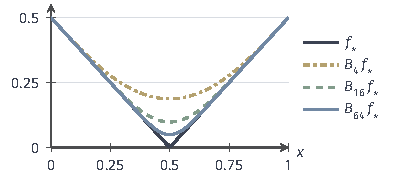
\includegraphics[width=66.7mm]{figures/02-abstract-mathematics/03-function-spaces/tikz/c6-bernstein-approx/figure.pdf}
  \caption{折线$f_*(x)=\lvert x-1/2\rvert$（黑）及其Bernstein多项式$B_4f_*$、$B_{16}f_*$、$B_{64}f_*$。每条曲线都是结点值的凸组合，位于$f_*$上方；一致误差都在$x=1/2$处取得，依次为$0.1875$、$0.0982$、$0.0497$，次数每增至四倍，误差约减半。}
  \label{fig:fapprox-bernstein}
\end{figure}

\paragraph{附加光滑性与误差速率}
定理保证$f_*$能被多项式任意逼近，但任何多项式都不等于$f_*$，因为多项式处处可微。“能任意逼近”与“给定次数下误差多大”是两个问题，后者需要对目标另加定量条件。若$f$是$L$-Lipschitz的，不必作近远分解，直接用Cauchy--Schwarz不等式与式~\eqref{eq:fapprox-bernstein-variance}：
\[
  \lvert B_mf(x)-f(x)\rvert\leq L\sum_j\Bigl\lvert\frac jm-x\Bigr\rvert w_{m,j}(x)\leq L\Bigl(\sum_j\Bigl(\frac jm-x\Bigr)^2w_{m,j}(x)\Bigr)^{1/2}\leq\frac L{2\sqrt m}.
\]
对$f_*$，$L=1$，界在$m=4,16,64$时为$0.25$、$0.125$、$0.0625$，与图~\ref{fig:fapprox-bernstein}中的实际误差同阶。对$\sqrt x$只有$\lvert f(s)-f(t)\rvert\leq\lvert s-t\rvert^{1/2}$，同样的论证（先对$\lvert j/m-x\rvert^{1/2}$用Cauchy--Schwarz）只给出$(4m)^{-1/4}$。条件越弱，这一构造能保证的速率越慢。

更多的光滑性并不能让Bernstein多项式更快。由引理~\ref{lem:fapprox-bernstein-moments}，$B_m(x^2)=x^2+x(1-x)/m$，误差恰为$1/(4m)$量级，而$x^2$本身就是二次多项式，$m\geq2$时最佳误差为零。所以Bernstein构造给出的是对所有连续函数都可验证的收敛机制，不是给定次数下的最佳近似。对最佳多项式逼近误差$E_m(f)=E(f,\mathcal P_m)_\infty$，其中$\mathcal P_m$是次数至多$m$的多项式空间，Jackson型定理给出：若$f\in C^r[a,b]$，则$E_m(f)\leq C_rm^{-r}\omega_{f^{(r)}}(1/m)$，常数$C_r$只依赖$r$与区间。光滑性越高，最佳多项式误差下降越快；对只有折点的$f_*$，最佳误差按$1/m$下降，也不能更快。这两条结论这里都不给出证明。

多项式还有一个结构上的特点：它是全局的。改变一个系数，整个区间上的函数值都会改变；Bernstein权重也在整个$(0,1)$上非零。目标若只在一处不光滑，例如$f_*$的折点，这一处的困难会影响全区间上的近似。下一小节的分段表示把这种影响限制在局部。

\subsection{固定网格上的分段逼近}
\label{sec:fapprox-fixed-grid}

另一种思路是先把区间切成小段，每段只用低次多项式。固定结点$0=t_0<t_1<\cdots<t_N=1$，记网格尺寸$h=\max_i(t_{i+1}-t_i)$。网格在看到目标之前就已经选定，所以候选集合仍是固定的线性空间；预算由单元数$N$和每个单元内的次数共同决定。

\paragraph{分段常数与分段多项式}
最简单的选择是每个单元上取常数。若在单元$[t_i,t_{i+1}]$上取该单元内函数值的最佳常数$(\max+\min)/2$，由第~\ref{sec:fapprox-fixed-space}节，单元上的误差为振幅的一半，因此整体一致误差不超过$\omega_f(h)/2$。若$f\in C^1$，振幅不超过$h\lVert f'\rVert_\infty$，误差至多$h\lVert f'\rVert_\infty/2$，按一阶下降。

每个单元上用$r$次多项式、单元之间不加任何衔接条件时，空间维数为$N(r+1)$。若$f\in C^{r+1}[0,1]$，在每个单元上取$f$在中点$c_i$处的$r$次Taylor多项式，由Taylor余项，单元内
\[
  \lvert f(x)-p_i(x)\rvert\leq\frac{\lVert f^{(r+1)}\rVert_\infty}{(r+1)!}\Bigl(\frac h2\Bigr)^{r+1}.
\]
误差按$h^{r+1}$下降。这是一个可验证的构造，不必是该空间中的最佳近似；它说明提高单元内次数换来的是更高的阶，前提是目标有相应阶的有界导数。

\paragraph{分段线性插值}
在实际中更常用的是连续的分段线性函数。对$x\in[t_i,t_{i+1}]$，令
\begin{equation}
  S_hf(x)=(1-s)f(t_i)+s\,f(t_{i+1}),\qquad s=\frac{x-t_i}{t_{i+1}-t_i}\in[0,1].
  \label{eq:fapprox-linear-interpolant}
\end{equation}
相邻两段在公共结点取同一个值，所以$S_hf$是经过全部结点值的连续折线，称为$f$的\term{分段线性插值}（piecewise linear interpolation）。在每段上为一次函数的全体连续函数组成$N+1$维空间。对每个结点$t_i$，令$\varphi_i$为在$t_i$处取$1$、在其余结点取$0$的连续折线，它在$[t_{i-1},t_{i+1}]$上呈三角形，称为\term{帽形函数}（hat function）。于是$S_hf=\sum_if(t_i)\varphi_i$，系数就是结点值。

\begin{theorem}[分段线性插值的误差]
\label{thm:fapprox-linear-interpolation}
若$f\in C[0,1]$，则$\lVert f-S_hf\rVert_\infty\leq\omega_f(h)$。若进一步$f\in C^2[0,1]$，则
\begin{equation}
  \lVert f-S_hf\rVert_\infty\leq\frac{h^2}8\lVert f''\rVert_\infty .
  \label{eq:fapprox-interpolation-quadratic}
\end{equation}
\end{theorem}

\begin{proof}
在单元$[t_i,t_{i+1}]$上，$f(x)-S_hf(x)=(1-s)\bigl(f(x)-f(t_i)\bigr)+s\bigl(f(x)-f(t_{i+1})\bigr)$。$x$到两端点的距离都不超过$h$，两个差值都不超过$\omega_f(h)$，凸组合也不超过$\omega_f(h)$。

再证二阶界。固定单元内一点$x\in(t_i,t_{i+1})$，令$g=f-S_hf$，它在两端为零。取
\[
  \kappa=\frac{g(x)}{(x-t_i)(x-t_{i+1})},\qquad G(u)=g(u)-\kappa(u-t_i)(u-t_{i+1}),
\]
则$G$在$t_i,x,t_{i+1}$三点为零。两次使用Rolle定理，存在$\xi$使$G''(\xi)=0$。$S_hf$在单元内是一次函数，$G''(\xi)=f''(\xi)-2\kappa$，故
\[
  f(x)-S_hf(x)=\frac{f''(\xi)}2(x-t_i)(x-t_{i+1}).
\]
单元上$\lvert(x-t_i)(x-t_{i+1})\rvert\leq(t_{i+1}-t_i)^2/4\leq h^2/4$，代入即得。
\end{proof}

两个界依据不同。连续模界只用了凸组合，对任何连续目标都成立，也不要求等距：只要网格尺寸$h\to0$，插值就一致收敛。二阶界多用了$f''$的有界性，换来$h^2$的速率。常数$1/8$不能改进：取$f(x)=x^2$与两个结点$0,1$，误差$x-x^2$在$1/2$处取到$1/4=h^2\lVert f''\rVert_\infty/8$。

\paragraph{局部正则性与网格位置}
二阶速率所需的光滑性不能省略。取等距结点$t_i=i/N$，$N$为奇数，此时$1/2$不是结点，而是某个单元的中点。$f_*$在这个单元两端的值都是$h/2$，插值在单元内恒为$h/2$，而$f_*(1/2)=0$；其余单元上$f_*$本身是直线，插值没有误差。所以$\lVert f_*-S_hf_*\rVert_\infty=h/2$，只按一阶下降。图~\ref{fig:fapprox-spline-rates}在对数坐标中比较了光滑目标$\sin(\pi x)$与$f_*$：前者的误差贴近二阶界，后者恰为$h/2$。

\begin{figure}[!htb]
  \centering
  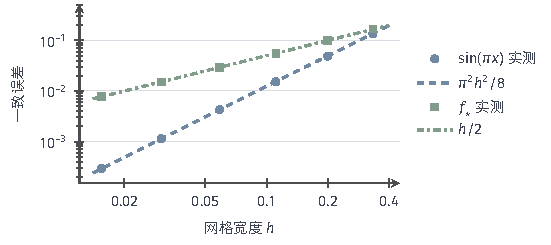
\includegraphics[width=93.4mm]{figures/02-abstract-mathematics/03-function-spaces/tikz/c6-spline-rates/figure.pdf}
  \caption{等距线性插值的一致误差与网格宽度$h=1/N$（$N=3,5,\ldots,65$为奇数，$1/2$不是结点），双对数坐标。光滑目标$\sin(\pi x)$的误差（圆点）贴近二阶界$\pi^2h^2/8$；折线$f_*$的误差（方块）恰为$h/2$，只按一阶下降。}
  \label{fig:fapprox-spline-rates}
\end{figure}

反过来，若结点恰好包含$1/2$，$f_*$在每个单元上都是直线，插值没有误差；用$t_0=0,t_1=1/2,t_2=1$三个结点就有$f_*=\frac12\varphi_0+0\cdot\varphi_1+\frac12\varphi_2$。同一个固定网格空间，对有的目标很有效，对稍微挪动了折点位置的目标就只剩一阶速率。固定网格的误差由目标在每个单元内的局部正则性决定，而折点落在哪个单元，在选网格时并不知道。这正是第~\ref{sec:fapprox-adaptive}节让分点随目标移动的动机。

\paragraph{拼接条件与维数}
单元之间的衔接条件改变维数，但不改变上面的阶。$N$个单元上不衔接的分段线性函数有$2N$维，要求连续后减少$N-1$个自由度，剩下$N+1$维，误差阶仍为$h^2$。更一般地，每段为$k$次多项式、在内部结点处$k-1$阶导数连续的函数称为$k$次\term{样条}（spline）。$N$段各有$k+1$个系数，$N-1$个内部结点各施加$k$个条件，维数为$(k+1)N-k(N-1)=N+k$；常用的三次样条维数为$N+3$。衔接条件让近似更光滑，并以较少的参数达到同样的阶，代价是系数与结点值不再一一对应，插值需要解一个线性方程组。

\paragraph{与全局多项式的比较}
在相同维数下比较两类空间。对光滑目标，维数为$N+1$的分段线性插值误差按$N^{-2}$下降，而次数为$N$的最佳多项式误差按Jackson型估计可以下降得更快；对$f_*$这类只在一点不光滑的目标，两者都只有一阶速率，但分段插值的误差只集中在含折点的一个单元里，其余单元上没有误差。全局多项式利用整体光滑性，分段多项式利用局部光滑性。选择哪一种，取决于目标的光滑性是整体的还是局部的。

\subsection{张量积表示}
\label{sec:fapprox-tensor}

目标有多个变量时，最自然的固定子空间是由一维表示相乘得到的。给定$x$方向的函数$\varphi_1,\ldots,\varphi_m$与$y$方向的函数$\psi_1,\ldots,\psi_n$，乘积$(\varphi_i\otimes\psi_k)(x,y)=\varphi_i(x)\psi_k(y)$称为两者的\term{张量积}（tensor product）。全体乘积的线性组合组成$mn$维空间（每组函数线性无关时），系数排成$m\times n$矩阵；有限维的张量积与Kronecker积可参考\BookChapterRef{chap:linear-operations}{卷二第1章“向量、矩阵与张量的运算”}。

\paragraph{网格插值与组合误差}
在$[0,1]$上取等距结点$t_i=i/(m-1)$，$i=0,\ldots,m-1$，帽形函数为$\varphi_0,\ldots,\varphi_{m-1}$，网格宽度$h=1/(m-1)$。二维插值取
\[
  (\Pi f)(x,y)=\sum_{i=0}^{m-1}\sum_{k=0}^{m-1}f(t_i,t_k)\,\varphi_i(x)\varphi_k(y).
\]
乘积$\varphi_i\otimes\varphi_k$支撑在一个矩形上，任一点只受它所在网格单元四个角点的影响，这就是双线性插值。图~\ref{fig:fapprox-tensor-grid}(a)画出$m=5$时一个乘积基的支撑与一个查询点所用的四个角点。

误差可以由一维结果逐个方向得到，但要多用一条性质。记$I_x$为固定$y$只对$x$作线性插值，$I_y$类似，则$\Pi=I_xI_y$。$I_x$是结点值的凸组合，所以$\lVert I_xg\rVert_\infty\leq\lVert g\rVert_\infty$。若$f\in C^2([0,1]^2)$，由定理~\ref{thm:fapprox-linear-interpolation}，
\[
  \lVert f-\Pi f\rVert_\infty\leq\lVert f-I_xf\rVert_\infty+\lVert I_x(f-I_yf)\rVert_\infty\leq\frac{h^2}8\bigl(\lVert\partial_x^2f\rVert_\infty+\lVert\partial_y^2f\rVert_\infty\bigr).
\]
第二项能用一维误差控制，靠的是$I_x$不放大一致范数；若某个方向的插值算子范数大于$1$，组合后的整体误差会被这个范数放大，单变量误差就不足以控制它。同样的论证在$d$维给出误差至多$d\,h^2\max_i\lVert\partial_i^2f\rVert_\infty/8$。

\paragraph{成本随维数的增长}
误差只随维数线性增大，所需系数个数却是$m^d$。设每个$\lVert\partial_i^2f\rVert_\infty\leq1$，要求误差不超过$\varepsilon=10^{-3}$，上式要求$h^2\leq8\varepsilon/d$。$d=2$时$h\leq0.0632$，取$m=17$，共$289$个系数；$d=6$时$h\leq0.0365$，需要$m=29$，共$29^6\approx5.9\times10^8$个系数。每个方向的分辨率只略有提高，总数却增长了六个数量级。这种由完整组合造成的规模增长称为\term{维数灾难}（curse of dimensionality）。第~\ref{sec:fapprox-fourier-truncation}节的多变量Fourier截断有同样的现象：保留$\max_i\lvert k_i\rvert\leq K$需要$(2K+1)^d$个系数。

\begin{figure}[!htb]
  \centering
  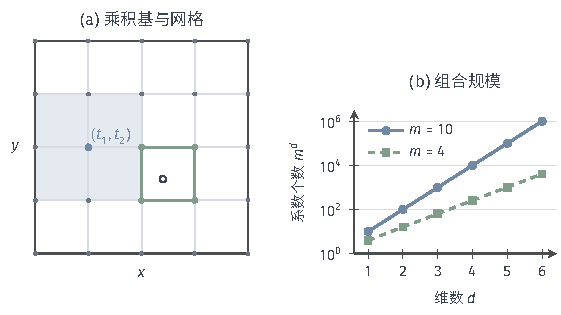
\includegraphics[width=95.0mm]{figures/02-abstract-mathematics/03-function-spaces/tikz/c6-tensor-grid/figure.pdf}
  \caption{张量积网格。(a)每轴$m=5$个结点，蓝底为乘积帽形基$\varphi_1(x)\varphi_2(y)$的支撑，蓝点为其中心结点$(t_1,t_2)$；空心圆为一个查询点，双线性插值只用它所在单元的四个角点（绿）。(b)完整张量积系数个数$m^d$随维数$d$指数增长（对数纵轴）。}
  \label{fig:fapprox-tensor-grid}
\end{figure}

比较成本时要写明计数的对象。上面数的是需要存储的系数，也就是网格上的函数值个数$m^d$；在一个点上求值只用所在单元的$2^d$个角点，代价随维数增长得慢得多；而确定这些系数需要的函数取样次数又与系数个数相同。“维数灾难”指的是前一种计数在固定误差要求下的指数增长，它来自对每个方向都使用同样分辨率的完整组合，并不说明所有多变量逼近都必须付出这样的代价。
